
\documentclass[11pt]{article}

\usepackage{graphicx}
\usepackage{framed}
\usepackage{listings}
\usepackage{titlesec}
\usepackage{tikz}
\usepackage{amssymb}
\usepackage{amsmath}
\usepackage{MnSymbol}
\usepackage{stmaryrd}

\newcommand{\sectionbreak}{\clearpage}

\lstset{frame=tb,
  language=Java,
  aboveskip=5mm,
  belowskip=5mm,
  showstringspaces=false,
  columns=flexible,
  basicstyle={\small\ttfamily},
  numbers=none,
  breaklines=true,
  breakatwhitespace=true
  tabsize=3
}


\newtheorem{theorem}{Theorem}[section]
\newtheorem{lemma}[theorem]{Lemma}
\newtheorem{proposition}[theorem]{Proposition}
\newtheorem{corollary}[theorem]{Corollary}

\newenvironment{proof}[1][Proof]{\begin{trivlist}
\item[\hskip \labelsep {\bfseries #1}]}{\end{trivlist}}
\newenvironment{definition}[1][Definition]{\begin{trivlist}
\item[\hskip \labelsep {\bfseries #1}]}{\end{trivlist}}
\newenvironment{example}[1][Example]{\begin{trivlist}
\item[\hskip \labelsep {\bfseries #1}]}{\end{trivlist}}
\newenvironment{remark}[1][Remark]{\begin{trivlist}
\item[\hskip \labelsep {\bfseries #1}]}{\end{trivlist}}



\newcommand{\qed}{\nobreak \ifvmode \relax \else
      \ifdim\lastskip<1.5em \hskip-\lastskip
      \hskip1.5em plus0em minus0.5em \fi \nobreak
      \vrule height0.75em width0.5em depth0.25em\fi}
\newcommand{\pre}{\mathop{\mathrm{pre}}}
\newcommand{\myparagraph}[1]{\paragraph{#1}\mbox{}\\}



\begin{document}

\tableofcontents
\section*{Abstract}

\section{Introduction}

\subsection{The Problem}

We are becoming increasingly dependent on computer systems. Not only are they an essential part of our lives, ...vital!



\subsection{The Idea}

\subsection{The Deliverables}


\begin{itemize}
\item Autonomous systems, what they are, why they are useful, and why they are vulnerable but we need to make sure they are reliable.
\item Verifying autonomous systems: what it entails, how we go about it (methods) and what are the challenges
\item The state explosion problem
\item Our idea and contributions
\item structure of the report
\end{itemize}

\section{Background}

\subsection{Logics for Multi-Agent Systems}

\subsubsection{Multi-Agent Systems}

Autonomous multi-agent systems are computer systems which are made up of several intelligent ``agents" acting within an ``environment". 
Intuitively, an \textit{agent} is: 
\begin{itemize}
\item Capable of \textit{autonomous} action 
\item Capable of \textit{social} interaction with its peers
\item Acting to \textit{meet} their design objectives 
\end{itemize}
 
Suppose we have a multi-agent systems consisting of $n$ agents and an environment $e$.
\begin{definition} 
An agent $i$ in the system consists of: 
\begin{itemize}
\item A set $L_i$ of local states representing the different configurations of the agent,
\item A set $Act_i$ of local actions that the agent can take,
\item A protocol function $P_i : L_i \rightarrow 2^{Act_i} $ expressing the decision making of the agent.
\end{itemize} 
\end{definition}

We can define the environment $e$ as a similar structure $(L_e, Act_e, P_e)$ where $P_e$ represents the functioning conditions of the environment. 

\subsubsection{Interpreted Systems}
\label{IS}
We present a formal structure to represent multi-agent systems. Consider a multi-agent system $\Sigma$ consisting of $n$ agents $1, ..., n$ and an environment $e$.
\begin{definition}
An \textit{Interpreted System} $IS$ for $\Sigma$ is a tuple $(G, \tau, I, \sim_1, ..., \sim_n, \pi)$, where
\begin{itemize}
\item $G \subseteq L_1 \times ... \times L_n \times L_e$ is the set of global states that $\Sigma$ can reach. A global state $g \in G$ is essentially a picture of the system at a given point in time, and the local state of agent $i$ in $g$ is denoted $l_i(g)$.
\item $I \subseteq G$ is a set of intial states for the system
\item $\tau : G \times Act \rightarrow G $ where $Act = Act_1 \times ... \times Act_n \times Act_e$ is a deterministic transition function (we can define $\tau : G \times Act \rightarrow 2^G$ to model a non-deterministic system)
\item $\sim_1, ..., \sim_n \subseteq G \times G$  are binary relations defined by $$g \sim_i g' \Leftrightarrow l_i(g) = l_i(g') \quad \forall g, g' \in G, \forall i = 1, ..., n$$
i.e iff agent $i$ is in the same state in both $g$ and $g'$. 
\item $\pi : PV \rightarrow G$ is a valuation function for the set of atoms $PV$, i.e for each atom $p \in PV$, $\pi(p)$ is the set of global states where $p$ is true
\end{itemize}
\end{definition}
We also need a formal definition for the ``execution'' of a system. A \emph{run}, as defined below, represents one possible execution of a MAS. 
\begin{definition} 
A \emph{run} of an interpreted system $IS = (G, \tau, I, \sim_1, ..., \sim_n, \pi)$ is a sequence $r = g_0, g_1, ...$ where $g_0 \in I$ and such that for all $i \geq 0$, $\exists a \in Act$ such that $\tau(g_i, a) = g_{i+1}$.
\end{definition}

Interpreted systems as defined above are used as semantic structures for a particular family of logics, presented in the next section.

\subsubsection{Linear Temporal Logic} 
\label{LTL}

In order to verify properties of multi-agent systems, we first need to find a logic allowing us to describe these properties accurately. 

A good candidate is the Linear Temporal Logic (LTL), a modal temporal logic in which one can write formulas about the future of \emph{paths}. Here we use paths to represent infinite runs of an interpreted system. 

\begin{definition} 
The syntax of LTL formulas is given by the following BNF: 
$$\varphi := p \mid \lnot\varphi \mid \varphi \land \varphi \mid X\varphi \mid G\varphi \mid \varphi U\varphi$$
\end{definition}

The intuitive meanings of $X\varphi, G\varphi$ and $\varphi U\psi$ are respectively 
\begin{itemize} 
\item $\varphi$ holds at the ne\textbf{X}t time instant
\item $\varphi$ holds forever (\textbf{G}lobally)
\item $\varphi$ holds \textbf{U}ntil $\psi$ holds  
\end{itemize}

We define the unary operator $F$ to be the dual of $G$, i.e $F\varphi := \lnot G\lnot\varphi$ for any LTL formula $\varphi$. $F\varphi$ represents the idea that $\varphi$ will hold at some point in the \textbf{F}uture.   

\myparagraph{Semantics} 

A model for LTL is a Kripke model $M = (W, R, \pi)$ such that the relation $R$ is serial, i.e $\forall u \in W,  \exists v \in W$ such that $(u, v) \in R$.
The worlds in $W$ are called the \textit{states} of the model. 

\begin{definition} 
A \textit{path} in an LTL model $M = (W, R, \pi)$ is an infinite sequence of states $\rho = s_0, s_1, ...$ such that $(s_i, s_{i+1}) \in R$ for any $i \geq 0$.
We denote $\rho^i$ the suffix of $\rho$ starting at $i$ (note that $\rho^i$ is itself a path since $\rho$ is infinite).
\end{definition}

It is easy to see how such a model can be used to represent a computer system, and how an execution of this system can be written as a path.

 Our objective is to be able to verify that a system $S$ has property $P$, so if we encode $P$ as an LTL formula $\varphi_P$ and $S$ as a model $M_S$, then we need to be able to check whether $\varphi_P$ is \textit{valid} in $M$ (or at least true in a set of initial states). This technique is called \textit{model checking}, and we do this by using the following definition for the semantics of LTL:
\label{model_checking}

\begin{definition}
Given LTL formulae $\varphi$ and $\psi$, a model $M$ and a state $s_0 \in W$, we say that
\begin{eqnarray*}
(M, s_0) \models p &\Leftrightarrow& s_0 \in \pi(p) \\  
(M, s_0) \models \lnot \varphi &\Leftrightarrow& (M, s_0) \nmodels \lnot \varphi\\
(M, s_0) \models \varphi \land \psi &\Leftrightarrow& (M, s_0) \models \varphi \mbox{ and  } (M, s_0) \models \psi \\
(M, s_0) \models X\varphi &\Leftrightarrow& (M, s_1) \models \varphi \mbox{  for all states } s_1 \mbox{ such that } R(s_0, s_1)\\
(M, s_0) \models G\varphi &\Leftrightarrow& \mbox{for all paths } \rho = s_0, s_1, s_2, ... , \mbox{ we have } (M, s_i) \models \varphi \quad \forall i \geq 0 \\
(M, s_0) \models \varphi U\psi &\Leftrightarrow& \mbox{for all paths } \rho = s_0, s_1, s_2, ..., \exists j \geq 0 \mbox{ such that }  (M, s_j) \models \psi \\ && \mbox{ and }  (M, s_k) \models \varphi \quad \forall 0 \leq k < j
\end{eqnarray*}

\end{definition}
The expressive power of LTL is limited to quantification over \textit{all} possible paths. For example: 

\begin{itemize}
\item $FG($deadlocked$)$ 

In every possible execution, the system will be permanently deadlocked.


\item $GF($crash$)$

Whatever happens, the system will crash infinitely often.
\end{itemize}
Hence some properties cannot be expressed in LTL, as in certain applications we might want to quantify explicitely over paths. The Computation Tree Logic (CTL) can express this. 

\subsubsection{Computation Tree Logic} 

\begin{definition} 
The syntax of CTL formulae is defined as follows: 
$$ \varphi := p \mid \lnot \varphi \mid \varphi \land \varphi \mid EX\varphi \mid EG\varphi \mid E(\varphi U \varphi)$$
\end{definition}

Intuitively, $ EX\varphi,  EG\varphi,$ and $ E(\varphi U \psi)$ represent the fact that there exists a possible path starting from the current state such that, respectively, $\varphi$ is true at the next state, $\varphi$ holds forever in the future, and $\varphi$ holds until $\psi$ becomes true.

The dual operator $AX\varphi := \lnot EX \lnot\varphi $ can be used to represent the fact that in all possible paths from the current state, $\varphi$ is true at the next state.
Connectives $AG\varphi, AF\varphi,$ and $A(\varphi U\psi)$ can be defined in the same way. 

We also use models (as defined in \ref{LTL}) for the semantics of CTL, as follows:

\begin{definition} 
Given CTL formulas $\varphi$ and $\psi$, a model $M = (W, R, \pi)$ and a state $s_0 \in W$, the satisfaction of formulas at $s_0$ in $M$ is defined inductively as follows: 
\begin{eqnarray*}
(M, s_0) \models p &\Leftrightarrow& s_0 \in \pi(p) \\  
(M, s_0) \models \lnot \varphi &\Leftrightarrow& (M, s_0) \nmodels \lnot \varphi\\
(M, s_0) \models \varphi \land \psi &\Leftrightarrow& (M, s_0) \models \varphi \mbox{ and  } (M, s_0) \models \psi \\
(M, s_0) \models EX\varphi &\Leftrightarrow& \exists \mbox{ a path } s_0, s_1, s_2, ... \mbox{ such that } (M, s_1) \models \varphi \\
(M, s_0) \models EG\varphi &\Leftrightarrow& \exists \mbox{ a path } s_0, s_1, s_2, ... \mbox{ such that } (M, s_i) \models \varphi \quad \forall i \geq 0\\
(M, s_0) \models E(\varphi U\psi) &\Leftrightarrow&  \exists \mbox{ a path } s_0, s_1, s_2, ... \mbox{ for which } \exists i \geq 0 \mbox{ such that }  (M, s_i) \models \psi \\ && \mbox{ and }  (M, s_j) \models \varphi \quad \forall 0 \leq j < i
\end{eqnarray*}
\end{definition}
The quantifiers allow for more properties to be expressed, for example:
\begin{itemize}

\item $EF(AG($deadlocked$))$

It is possibly to reach a point where the process will be permanently deadlocked.

\item $AG(EX($reboot$))$ 

From any state it is possible to reboot the system.


\end{itemize}
Again, some formulas can be expressed in LTL but not in CTL. For instance, the property that \textit{in every path where $p$ is true at some point then $q$ is also true at some point} is expressed in LTL as $Fp \rightarrow Fq $ but there is no equivalent CTL formula.
 The logic CTL* combines the syntax of LTL and CTL to provide a richer set of connectives. We will not go into any more details regarding CTL*, but we refer the reader to \cite{ctl*} for more information. 

\subsubsection{The Epistemic Logic CTLK}

In the case of multi-agent systems, we are interested in describing the system in terms of individual agents, and in particular their \textit{knowledge}. 

For this reason, we can add \cite{ctlk} a family of unary operators $K_i$ for $i = 1, ..., n$ to the modal connectives defined previously. Each $K_i$ will represent the intuitive notion of knowledge for agent $i$. 
This enables us to define the temporal-epistemic logics LTLK and CTLK, which are extensions of LTL and CTL, respectively. Here we leave out details about LTLK, as the practical applications we present later on only support CTLK. 



\begin{definition} 
The syntax of CTLK is defined by the following BNF: 
$$ \varphi := p \mid \lnot \varphi \mid \varphi \land \varphi \mid EX\varphi \mid EG\varphi \mid E(\varphi U \varphi) \mid  K_i\varphi \quad (i \in \{1, ..., n\})$$
\end{definition}  

We use interpreted systems (\ref{IS}) as semantic structures for CTLK. The satisfaction of a CTL formula on an interpreted system $IS$ is defined analogously to its satisfaction on a model $M$ whose worlds $W$ are the global states of $IS$, and whose relation function $R$ is the global transition function of $IS$. 
For example, $(IS, g_0) \models EX\varphi \mbox{  iff there is a run } r = g_0, g_1, g_2, ... \mbox{ of $IS$ such that } (IS, g_1) \models \varphi$.

The following definition completes the semantics of CTLK formulae:

\begin{definition}
Given an interpreted system $IS$, a global state $g$, an agent $i$ of $IS$, and a CTLK formula $\varphi$, we define
$$(IS, g) \models K_i \varphi \mbox{  iff  } \forall g' \in G, g \sim_i g' \Rightarrow (IS, g') \models \varphi$$

The connective $K_i$ expresses that agent $i$ \emph{knows} of the property $\varphi$ when the system's global state is $g$.

We extend the syntax and semantics of CTLK by adding two extra unary operators: $E$ (Everybody knows) and $C$ (Common knowledge), whose semantics are defined as follows:

\begin{eqnarray*}
(IS, g_0) \models E\varphi &\Leftrightarrow& (IS, g_0) \models K_i \varphi \quad \forall i = 1, ..., n \\
(IS, g_0) \models C\varphi &\Leftrightarrow&  (IS, g_0) \models \bigwedge^\infty_{k = 1} E^{(k)}\varphi \quad \\&& \mbox{ where } E^{(1)} = E \mbox{ and } E^{(j+1)} = EE^{(j)} \quad \forall j \geq 1
\end{eqnarray*}
\end{definition}


\subsection{Model Checking}

Model checking was briefly introduced in \ref{model_checking} as a automated verification technique, which can be used to check that a system $S$ satisfies a specification $P$. The technique involves representing $S$ as a logic system $L_S$ which captures all possible computations of $S$, and encoding the property $P$ as a temporal formula $\varphi_P$. 

The problem of verifying $P$ is then reduced to the problem of checking whether $L_S \vdash \varphi_P $. But we can now build a Kripke model $M_S = (W_S, R_S, \pi)$ such that $L_S$ is sound and complete over (the class of) $M_S$, so that $$L_S \vdash \varphi_P \Leftrightarrow M_S \models \varphi_P .$$ 
$M_S$ is the Kripke model representing all possible computations of $S$, i.e. $W_S$ contains all the possible computational states of the system and the relation $R_S$ represents all temporal transitions in the system. 

In the case of a multi-agent system as defined above, encoding $S$ as an interpreted systems of agents will satisfy the equivalence, and we can use CTLK to encode properties of the system to be checked. 

\subsubsection{Explicit Model Checking}

\label{explicit}
In this section we present a first approach to model checking, the so-called \textit{explicit} approach.

Suppose that we want to check that a multi-agent system $\Sigma$ satisfies a propery $P$. If $IS$ is an interpreted system representing $\Sigma$, and $\varphi$ the CTLK formula corresponding to $P$, we need to verify that $(IS, s_0) \models \varphi$, for all initial states $s_0 \in I$.

Algorithmically it is more efficient \cite{need ref} to compute the set of global states $\llbracket\varphi\rrbracket$ of $IS$ where $\varphi$ is true, and check that $I \subseteq \llbracket\varphi\rrbracket$. 
The following algorithm returns $\llbracket\varphi\rrbracket$ for any CTLK formula $\varphi$.


\begin{lstlisting}[mathescape]

function SAT($\varphi$) 
// returns $\llbracket\varphi\rrbracket$
if $\varphi = \top$: return $G$
if $\varphi = \bot$: return $\varnothing$
if $\varphi = p$: return $\pi(p)$ 
if $\varphi = \lnot\varphi_1$: return $G \setminus$SAT($\varphi_1$)
if $\varphi = \varphi_1\land\varphi_2$: return SAT($\varphi_1$)$\cap$SAT($\varphi_2$)
if $\varphi = EX\varphi_1$: return SAT$_{\mbox{EX}}(\varphi_1)$
if $\varphi = AF\varphi_1$: return SAT$_{\mbox{AF}}(\varphi_1)$
if $\varphi = E(\varphi_1 U\varphi_2 )$: return SAT$_{\mbox{EU}}(\varphi_1, \varphi_2)$
if $\varphi = K_i\varphi_1$: return SAT$_{\mbox{K}}(i, \varphi_1)$
if $\varphi = E\varphi_1$: return SAT$_{\mbox{E}}(\varphi_1)$
if $\varphi = C\varphi_1$: return SAT$_{\mbox{C}}(\varphi_1)$
end
$\\$
\end{lstlisting}

Notice that this covers all formulae $\varphi$, as $\{EX, AF, EU, K_i, E, C\}$ is a minimum set of connectives for CTLK. The respective auxilliary functions are defined below. Notation: for any global states $g_0, g_1$ of $IS$ we write $g_0 \rightarrow g_1$ iff $\exists a \in Act$ such that $\tau(g_0, a) = g_1$ (i.e. there is an run of $IS$ starting with $g_0, g_1, ...$).


\begin{lstlisting}[mathescape]

function SAT$_{\mbox{EX}}$($\varphi$)
// returns $\llbracket EX\varphi\rrbracket$
  X := {$g_0 \in G \mid g_0 \rightarrow g_1$ for some $g_1 \in $SAT($\varphi$) }
  return X
end
 
function SAT$_{\mbox{AF}}$($\varphi$)
// returns $\llbracket AF\varphi\rrbracket$
  X := $G$
  Y := SAT($\varphi$)
  repeat until X = Y:
    X := Y
    Y := Y $\cup$ $\{ g_0 \in G \mid $ for all $g_1 $ with $g_0 \rightarrow g_1$, $g_1 \in$ Y $\}$ 
  end
  return Y
end
  

function SAT$_{\mbox{EU}}$($\varphi_1$, $\varphi_2$)
// returns $\llbracket E(\varphi_1U\varphi_2)\rrbracket$
  W := SAT($\varphi$)
  X := $G$
  Y := SAT($\psi$)
  repeat until X = Y:
    X := Y
    Y := Y $\cup$ (W $\cap$ $\{g_0 \in G \mid \exists g_1 \in$ Y such that $g_0 \rightarrow g_1\}$)
  end
  return Y
end

function SAT$_{\mbox{K}}$($i$, $\varphi$)
// returns $\llbracket K_i\varphi\rrbracket$
  X := SAT($\lnot\varphi$)
  Y := $\{g_0 \in G \mid \exists g_1 \in$ X with $g_0 \sim_i g_1\}$
  return $G \setminus\mbox{Y}$
end

function SAT$_{\mbox{E}}$($\varphi$)
// returns $\llbracket E\varphi\rrbracket$
  X := SAT($\lnot\varphi$)
  Y := $\{g_0 \in G \mid \exists g_1 \in$ X with $g_0 \sim_i g_1$ for all $i = 1, ..., n\}$
  return $G \setminus\mbox{Y}$
end

function SAT$_{\mbox{C}}$($\varphi$)
// returns $\llbracket C\varphi\rrbracket$
  X := $G$
  Y := SAT($\lnot\varphi$)
  repeat until X = Y:
    X := Y
    Y := $\{g_0 \in G \mid \exists g_1 \in$ X with $g_0 \sim_i g_1$ for all $i = 1, ..., n\}$
  end
  return $G \setminus\mbox{Y}$
end
$\\$
\end{lstlisting}
The complexity of \texttt{SAT} is linear in the size of the model. However, the size of the model (i.e. the number of reachable states) grows exponentially in the number of variables used to describe the system $\Sigma$, therefore the explicit approach is not always viable in practice. This is the main difficulty in model checking and it is known as the \textit{state explosion problem}. 

Recall that in order to use the algorithm above we also need a way of computing the set of reachable states, which is rarely given explicitely. In most cases all that is given is the set $I$ of initial states of the system. The reachable state space can then be obtained by computing the fixed point of the transition relation function, as shown in the algorithm below:

\begin{lstlisting}[mathescape]

function compute_reach()
// returns the reachable state space $G$ 
  X := $\emptyset$
  Y := $I$
  repeat until X = Y
    X := Y
    Y := Y $\cup$  $\{ g_1 \in G \mid g_0 \rightarrow g_1 \mbox{ for some }g_0 \in X\}$
  end
  return Y
end
$$
\end{lstlisting}

In the next section we introduce a model checking technique aiming to improve the efficiency of the approach. 



\subsubsection{Symbolic Model Checking}

\textit{Symbolic model checking} is an approach to model checking which involves representing sets of states and functions between them as Boolean formulas. The algorithm presented in \ref{explicit} is then reduced to a series of operations on Boolean formulas. In this section we go through the process of encoding sets and functions as propositional formulas, and we explain how this encoding facilitates model checking.

\myparagraph{Symbolic Representation of Sets of States}
\label{symbolic}
\begin{figure}
    \centering
    \includegraphics[scale=0.55]{symbolic_model_checking_example.PNG}
    \caption{A model}
    \label{fig:model_example}
\end{figure}

We use an example \cite{logic_in_computer_science} to illustrate the encoding process.
Consider the model in Figure~\ref {fig:model_example}, representing a system with three states labelled $s_0, s_1, s_2$. 

We consider two propositional variables, namely $x_1$ and $x_2$.  
If $S$ is the whole state space (so $S = \{s_0, s_1, s_2\}$), we can represent subsets of $S$ using Boolean formulae, as shown in the following table:\\

\begin{tabular}{ l | r }
  set of states & representation by boolean formula \\ \hline
$\emptyset $&   $\bot$ \\
$\{ s_0\}$ & $x_1 \land \lnot x_2 $\\
$\{ s_1\}$ & $ \lnot x_1 \land x_2 $\\
$\{ s_2\}$ & $\lnot x_1 \land \lnot x_2 $\\
$\{ s_0, s_ 1\}$ & $(x_1 \land \lnot x_2) \lor (\lnot x_1 \land x_2)  $\\
$\{ s_1, s_2\}$ & $(\lnot x_1 \land  x_2) \lor (\lnot x_1 \land\lnot x_2)$\\
$\{ s_0, s_2\}$ & $(x_1 \land \lnot x_2) \lor (\lnot x_1 \land\lnot x_2) $\\
$\{ s_0, s_1, s_2\}$ & $(x_1 \land \lnot x_2) \lor (\lnot x_1 \land  x_2) \lor (\lnot x_1 \land\lnot x_2)$
\end{tabular}
\\
\\

Note that for this representation to be unambiguous, we must ensure that no two states satisfy the same set of Boolean variables. If this is the case, new variables can be added which will be used to differenciate between the ambiguous states.


\myparagraph{Symbolic Representation of a Transition Relation}

The transition relation $\rightarrow$ of a model is a subset of $S \times S$. Taking two copies of our set of propositional variables, we can then associate a Boolean formula to the transition relation, as follows. 

Firstly, notice that in the example above the transition relation $\rightarrow$ of the model is $$\{(s_0, s_1), (s_1, s_2), (s_2, s_0), (s_2, s_2)\}.$$
Our set of Boolean variables was $\{x_1, x_2\}$; we now create a copy and use \textit{primed} variables to represent its elements. We get another set $\{x_1', x_2'\}$, which will be used to represent the \textit{next} state in our encoding of the transition relation.
Now, for each pair element in the set, we take the conjunction of the Boolean representation of each state in the pair, the first one using the original set of variables, the second the primed set. For example, with $(s_0, s_1)$ is associated the formula $(\lnot x_1 \land \lnot x_2) \land (\lnot x'_1 \land \lnot x'_2)$ (using the Boolean representation for $s_0, s_1$ derived above -- see the table).

As in the representation of sets of states, we represent sets of pairs by taking the conjunction of the representation of each pair element. Thus we compute the representation of $\rightarrow$ to be $(\lnot x_1 \land \lnot x_2 \land \lnot x'_1 \land \lnot x'_2 ) \lor (\lnot x_1 \land \lnot x_2 \land x'_1 \land \lnot x'_2 ) \lor ( x_1 \land \lnot x_2 \land \lnot x'_1 \land  x'_2 ) \lor (\lnot x_1 \land x_2 \land \lnot x'_1 \land \lnot x'_2 )$.

\myparagraph{The functions $\pre_\exists$ and $\pre_\forall$}

We have seen that the explicit model checking algorithm relies on two functions on sets of states, $$\mbox{pre}_{\exists} (X) = \{g_1 \in G \mid \exists g_0 \in X \mbox{ with } g_0 \rightarrow g_1\}$$ and $$\mbox{pre}_\forall (X) = \{g_1 \in G \mid\mbox{ if }g_0 \rightarrow g_1,\mbox{ then }g_0 \in X\}.$$ We therefore need a way of implementing those using the symbolic representations of sets of states introduced above. First note that $$\mbox{pre}_\forall (X) = G \setminus \mbox{pre}_{\exists} (G \setminus X),$$ so it is enough to have an algorithm for computing $\mbox{pre}_{\exists}(X)$ on a given set~$X$. Let us first recall a basic definition about Boolean functions:

\begin{definition}
\label{exist}
Let $f$ be a Boolean function. The \textit{conditioning} of $f$ on a variable $x$, written $f|_x$, is the Boolean function obtained by changing $x$ to $\top$ in $f$, and similarly $f|_{\lnot x}$
is obtained from $f$ by setting $x$ to $\bot$.
The \textit{existential quantification} of $f$ with respect to $x$, denoted $\exists x f$, is used to relax the constraint on variable $x$ in $f$, and it is defined by $$\exists x f = f|_x \lor f|_{\lnot x}.$$
\end{definition}

Suppose now that $X \subseteq G$ is a set of states encoded by function $f_X$, and that the transition relation $\rightarrow$ of the system is encoded by function $f_\rightarrow$. The algorithm has the following steps:
\begin{enumerate}
\item Rename variables in $f_X$ to their primed counterparts, and call the resulting function $f_{X'}$. 
\item Compute $f_{\rightarrow X'} = f_{X'} \land f_\rightarrow$.
\item Existentially quantify all primed variables away from $f_{\rightarrow X'}$, i.e. compute $\exists x_1' ... \exists x_n' f_{\rightarrow X'}.$ The resulting function is $f_{\mbox{pre}_\exists(X)}$, the symbolic representation of $\mbox{pre}_\exists(X)$.
\end{enumerate}
In the \texttt{compute\_reach} algorithm above, we use a different operator, which computes the set of states \textit{following} $X$ in the transition relation. This can be encoded in terms of Boolean functions in a very similar way: start with the Boolean encoding of $X$, conjoin with the encoding of the transition relation, existentially quantify all non-primed variables, and ``un-prime" the variables in the resulting function.

\myparagraph{The case of Multi-Agent Systems}

Notice that the procedure described above is only valid for global states and does not distinguish between different agents. 
In the case of multi-agent systems, we can encode the local states for agents using the same method as for states in the general case, making sure to use a different set of variable for each agent. A Boolean representation for a global state in the system will then be the conjunction of the formulas for the local states of which it consists. The separate encoding of the states for each agent will also enable the agent protocols to be encoded independently.

Moreover, in order to successfully implement our model checking algorithm using symbolic expressions, we need a way of representing the agent accessibility relations $\sim_i$.
But each of these is a binary relation on states, i.e. a subset of $S \times S$. Hence we can use the exact same method as for the global transition relation. 
\\\\

How does this help us? Well, several techniques exist which allow us to represent these Boolean formulas in a very concise form. This is the topic of the next section.

\subsection{Representing Boolean functions}

It is important to make the point that the Boolean formulas computed in \ref{symbolic} can be regarded as Boolean \textit{functions}, i.e. functions $\{0, 1\}^n \rightarrow \{0, 1\}$ for some $n$. For example, the formula $x_1 \land \lnot x_2$ is associated to the function $f(x_1, x_2) = x_1 \land \lnot x_2$.

In this section we introduce various representations of Boolean functions using directed acyclic graphs (DAG). 

\subsubsection{Ordered Binary Decision Diagrams}

One the most basic ways of representing a Boolean function is by using a \textit{binary decision tree} (BDT). A BDT is a binary tree where we label non-terminal nodes with Boolean variables $x_1, x_2, ...$ and terminal nodes with the values 0 and 1. Each non-terminal node has two outgoing edges, one solid and one dashed (one for each value of the variable the node is labelled with). An example is shown in Figure~\ref{fig:BDT}. Note that the initial ordering of the variables affects the resulting BDT; for convenience, we write $[x_1, x_2, ..., x_n]$ to denote the order $x_1 < x_2 < ... < x_n$.


BDTs are a relatively inefficient way of storing Boolean formulas, since a BDT for a formula with $n$ variables has $2^{n+1} - 1$ nodes. Fortunately, a BDT can be reduced to an \textit{ordered binary decision diagram} (OBDD), a much more compact data structure.

\begin{figure}
\centering
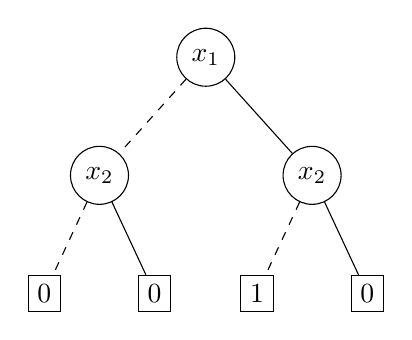
\begin{tikzpicture}

	\node[circle, draw] (x1) {$x_1$}	 [sibling distance=27mm]
		child {node[circle,draw] (x21) {$x_2$} [sibling distance=14mm][dashed]
			child {node[rectangle, solid, draw] (1) {0} [dashed]}
			child {node[rectangle, solid, draw] (01) {0} [solid]}}
		child {node[circle,draw] (x22) {$x_2$} [sibling distance=14mm][solid]
			child {node[rectangle, solid, draw] (02) {1} [dashed]}
			child {node[rectangle, solid, draw] (03) {0} [solid]}};
\end{tikzpicture}
	\caption{BDT for $f(x_1, x_2) = x_1 \land \lnot x_2$ under the ordering $[x_1, x_2]$}
\label{fig:BDT}
\end{figure}

\myparagraph{The Reduction Algorithm} 

\noindent There are three steps in the reduction of BDTs to OBDDs:
\begin{enumerate}
\item Removal of duplicate terminals: we merge all the 0-nodes and 1-nodes into two unique terminal nodes
\item Removal of redundant tests: if both outgoing edges of a node $n$ point to the same node $m$, we remove $n$ from the graph, sending all its incoming edges directly to $m$ 
\item Removal of duplicate non-terminals: we merge any two subtrees with identical BDD structure
\end{enumerate}
Steps (2) and (3) are repeatedly applied until no further reduction is possible, and the resulting diagram is said to be a reduced ordered binary decision diagram. 

[here need example of using reduction algorithm]

The following key result makes the use of OBDDs viable in practice: 

\begin{theorem} \cite{bryant}
\label{obdd_uniqueness}
If $f$ is a Boolean function over the variables $x_1, ..., x_n$, then the OBDD representing $f$ is unique, up to the order of $x_1, ..., x_n$ chosen.
\end{theorem}

The immediate consequence of Theorem~\ref{obdd_uniqueness} is that one can easily compare two Boolean functions by comparing their respective OBDDs (provided both OBDDs have the same variable order). 

Another important observation to make is that OBDDs resulting from two different variable orders may present a \textit{significant }difference in size, and therefore a large amount of work has been done in the search for suitable variable orders. 

OBDDs help us to manipulate Boolean functions with a high number of variables, allowing us to use our model checking algorithm (\ref{explicit}) on systems with much larger state-spaces, which has led researchers in the past 15 years to explore various graph-based representations of Boolean functions.

\noindent\textit{Note to the reader: throughout this report we often drop the `O' and refer to OBDDs as BDDs.}

\subsubsection{A Knowledge Compilation Map}

In computer science, the field of \textit{knowledge compilation} is concerned with finding compact and efficient representations of propositional knowledge bases (such as symbolic representations of state-spaces, cf \ref{symbolic}).
 Such a representation is refered to as a \textit{target compilation language}, of which BDTs and OBDDs are examples. 
 
 The main properties that we look for in a target compilation language are the canonicity of the representation, the succinctness of the representation, and a polynomial-time complexity for queries and operations on the language. 
 These properties will ensure that we can safely rely on a particular language for our model checking algorithm. 
 
 OBDDs satisfy these two properties (with succintness remaining highly dependent on the variable order), and in fact a number of model checkers use them for state-space representation (e.g. NuSMV, MCMAS). 
 
 In 2002, A. Darwiche and P. Marquis published \cite{compilation_map} a comparative analysis of most existing DAG-based target compilation languages in terms of their succintness and the polytime operations they support. They show that all of these languages are subsets of a broad language called \textit{negation normal form} (NNF). 

\begin{definition}
A sentence in \textit{NNF} is a rooted directed acyclic graph where each leaf node is labelled with $\top$, $\bot$, $X$ or $\lnot X$ for some propositional variable $X$, and each internal node is labelled with $\land$ or $\lor$ and can have arbitrarily many children. 

\end{definition} 

\noindent Remark: OBDDs are NNF sentences. Figure~\ref{nnf_obdd} shows an OBDD and its corresponding NNF sentence.  

\begin{figure}
\centering
\begin{tikzpicture}


	\node[circle, draw] (X) at (0, 5){$X$};
	\node[circle, draw] (Y) {$Y$};

\end{tikzpicture}
\qquad\quad
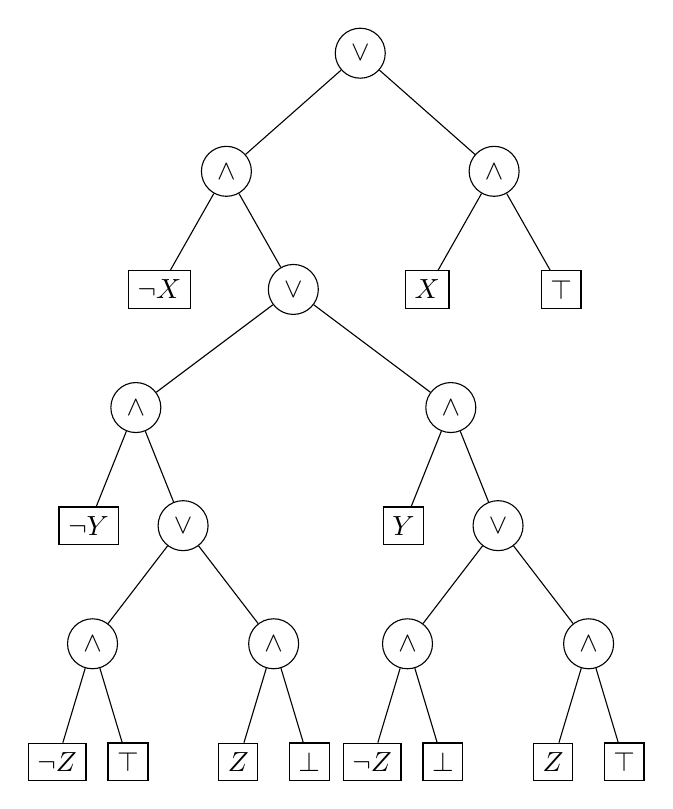
\begin{tikzpicture}
	[level 1/.style={sibling distance=34mm},
	 level 2/.style={sibling distance=17mm},
	 level 3/.style={sibling distance=40mm},
	 level 4/.style={sibling distance=12mm},
	 level 5/.style={sibling distance=23mm},
	 level 6/.style={sibling distance=9mm}]
	\node[circle, draw] (or1) {$\lor$}	 
		child {node[circle,draw] (and1) {$\land$} [solid]
			child {node[rectangle, solid, draw] (X1) {$\lnot X$}[solid]}
			child {node[circle, solid, draw] (or2) {$\lor$} [solid]
				child {node[circle,draw] (and3) {$\land$} [solid]
					child {node[rectangle, solid, draw] (Y1) {$\lnot Y$}[solid]}
					child {node[circle, solid, draw] (or5) {$\lor$} [solid]
						child {node[circle,draw] (and5) {$\land$} [solid]
							child {node[rectangle, solid, draw] (Z1) {$\lnot Z$}[solid]}
							child {node[rectangle, solid, draw] (T2) {$\top$} [solid]} 	
						}
						child {node[circle,draw] (and6) {$\land$} [solid]
							child {node[rectangle, solid, draw] (Z2) {$Z$}[solid]}
							child {node[rectangle, solid, draw] (F1) {$\bot$} [solid]} 	
						}
					}
				}
				child {node[circle,draw] (and4) {$\land$} [solid]
					child {node[rectangle, solid, draw] (Y2) {$Y$}[solid]}
					child {node[circle, solid, draw] (or6) {$\lor$} [solid]
						child {node[circle,draw] (and7) {$\land$} [solid]
							child {node[rectangle, solid, draw] (Z3) {$\lnot Z$}[solid]}
							child {node[rectangle, solid, draw] (F2) {$\bot$} [solid]} 	
						}
						child {node[circle,draw] (and8) {$\land$} [solid]
							child {node[rectangle, solid, draw] (Z2) {$Z$}[solid]}
							child {node[rectangle, solid, draw] (T2) {$\top$} [solid]} 	
						}
					}
				}
			}
		}
		child {node[circle,draw] (and2) {$\land$} [solid]
			child {node[rectangle, solid, draw] (X2) {$X$} [solid]}
			child {node[rectangle, solid, draw] (T1) {$\top$} [solid]}
		};
\end{tikzpicture}

	\caption{An OBDD (left) and its corresponding NNF sentence (right). Although the former seems much more compact, the difference in size is only linear and both representations are essentially the same. TODO sort this oout}
\label{nnf_obdd}

\end{figure}
 
 
 
\subsubsection{Project Directions}

 This ``knowledge compilation map" was the starting point for this project, whose initial objective was to investigate new target compilation languages suitable for application to model checking, seeking a potential improvement on BDDs (which constitute so far the ``industry standard").

 Taking into account the various criteria for suitable representations described above, we searched the literature aiming to find a good candidate to replace BDDs. 

After considering a number of different representations including tree-of-BDDs \cite{trees_of_bdds}, BDD-trees \cite{bdd_trees}, and several other subsets of NNF described in \cite{compilation_map}, we opted for a relatively novel target compilation language called \textit{sentential decision diagram} (SDD). 

SDDs are a subset of NNF, possess the required properties, and had not yet been experimented with in the context of model checking and state-space representation. 
Moreover, some of the experimental results presented in \cite{sdd_1} and \cite{sdd_3} demonstrate that SDDs can lead to a significant improvement on BDDs in terms of computation time and memory usage. 

In the next section we present SDDs in full details, delaying our own experimental results to the following chapters.


\subsection{Sentential Decision Diagrams}

Most of the content in that section is taken from the work of A. Darwiche in \cite{sdd_1}, the first paper written on SDDs. 

\subsubsection{Preliminaries}

To define SDDs formally we must start with some preliminary definitions and results related to Boolean functions. 

\begin{definition} 
We say that a function $f$ \textit{essentially depends} on a variable $x$ iff $f|_{x} \neq f|_{\lnot x}$, and we write $f(X)$ if $f$ essentially depends on variables in $X$ only.
\end{definition}

\noindent Notation: we also write $f(X, Y)$ if $f(Z)$ and $X$, $Y$ are sets forming a partition of $Z$.

The following definition is the basis for the construction of SDDs:

\begin{definition} (Decompositions and partitions)
An \textit{($X$,$Y$)-decomposition} of a function $f(X, Y)$ is a set of pairs $\{(p_1, s_1),...,(p_n, s_n)\}$ such that $$ f = (p_1(X) \land s_1(Y)) \lor ... \lor (p_n(X) \land s_n(Y)).$$
The decomposition is said to be \textit{strongly deterministic} on $X$ if $p_i(X) \land p_j(X) = \bot$ for $i \neq j$. In this case, each ordered pair $(p_i, s_i)$ in the decomposition is called an \textit{element}, each $p_i$ a \textit{prime} and each $s_i$ a \textit{sub}.

Let $\alpha = \{(p_1, s_1),...,(p_n, s_n)\}$ be an ($X,Y$)-decomposition, and suppose $\alpha$ is strongly deterministic on $X$.
Then $\alpha$ is called an $X$-\textit{partition} iff its primes form a partition (i.e primes are pairwise mutually exclusive, each prime is consistent, and the disjunction of all primes is valid).
We say that $\alpha$ is \textit{compressed} if $s_i \neq s_j$ for $i \neq j$.
\end{definition}

\begin{example} 
Let $f(x, y, z) = (x \land y) \lor (x \land z)$. Then $\alpha = \{(x, y\lor z)\}$ is an $(\{x\}, \{y, z\})$-decomposition of $f$ which is strongly deterministic (as there is only one prime). It is however not an $\{x\}$-partition, but $\beta = \{(x, y\lor z), (\lnot x, \bot)\}$ is, since $x, \lnot x$ form a partition. Note that $\beta$ is compressed. 
\end{example}

\noindent Remark that in an $X$-partition $\bot$ can never be prime, and if $\top$ is prime then it is the only prime. Moreover primes determine subs, so two $X$-partitions are different iff they contain distinct primes.

\begin{theorem}
\label{theorem_apply}
Let $\circ$ be a Boolean operator and let $\{(p_1, s_1),...,(p_n, s_n)\}$ and $\{(q_1, r_1),...,(q_m, r_m)\}$  be $X$-partitions of Boolean functions $f(X, Y)$ and $g(X, Y)$ respectively. Then $$\{(p_i \land q_j, s_i \circ r_j) \mid  p_i \land q_j  \neq \bot \}$$ is an $X$-partition of $f \circ g$.
\end{theorem}
\begin{proof}
 Since $p_1, ..., p_n$ and $q_1, ..., q_m$ are partitions, the $(p_i \land q_j)$ also form a partition for $i = 1, ..., n$, $j = 1, ..., m$ and $p_i \land q_j \neq \bot$. 
 
To do: finish proof 
\end{proof}

As we see later on, an important consequence of Theorem~\ref{theorem_apply} is the polynomial time operations available on SDDs. Canonicity of SDDs is due to the following result:

\begin{theorem}
\label{unique_compressed}
A function $f(X, Y)$ has exaclty one compressed $X$-partition.
\end{theorem}
\begin{proof}
proof
\end{proof}

\myparagraph{Vtrees}

Vtrees (for ``variable trees") are to SDDs what variable orders are to BDDs. A vtree completely determines the structure of an SDD, so they are crucial to the viability of SDDs in practice.

\begin{definition}
A \textit{vtree} for variables $X$ is a full binary tree whose leaves are in one-to-one correspondence with the  variables in $X$. We will often not distinguish between a vtree node $v$ and the subtree rooted at $v$, and the left and right children of a node $v$ will be denoted $v^l$ and $v^r$, respectively.
\end{definition}

\begin{figure}
\centering
\includegraphics[scale=0.5]{balancedABCD.png}
\qquad
\includegraphics[scale=0.5]{rightlinearABCD.png}


\caption{Two vtrees for $X = \{A, B, C, D\}$ To Do sort out nodes IDs}
\label{fig:vtree_examples} 

\end{figure}
Note that a vtree on a set $X$ is stronger than a total order of the variables in $X$. Figure~\ref{fig:vtree_examples} shows two distinct vtrees which induce the same variable order. 

\subsubsection{Definition and Construction}

The construction of an SDD for a Boolean function $f$ with respect to a vtree $v$ is done by a recursive algorithm on the children nodes of $v$. 

Let $v$ be the vtree on the left of Figure~\ref{fig:vtree_examples}, and let $$f(A, B, C, D) = (A \land B) \lor (B \land C) \lor (C \land D).$$

The decomposition of $f$ at the vtree node $v$ goes as follows: we split the variables in $X$ into two subsets by separating variables in $v^l$ from those in $v^r$: we obtain $\{A, B\}$ and $\{C, D\}$; we take the unique compressed $\{A, B\}$-partition of $f$, namely $\alpha = \{(\lnot B , C\land D), (\lnot A \land B, C), (A \land B, \top)\}$. The SDD for $f$ is the decomposition obtained by further decomposing the primes of $\alpha$ at $v^l$ and its subs at $v^r$. We continue this recursively until all elements consist of literals or constants. 

\myparagraph{Graphical Representation of SDDs}

The SDD constructed for function $f$ is represented on the left in Figure~\ref{fig:sddexample1}. On the right is the SDD for $f$ constructed with respect to the vtree on the right in Figure~\ref{fig:vtree_examples}.

A decomposition is represented by a circle with outgoing edges pointing to its elements, and an element is represented by a pair of boxes where the left box represents the prime and the right box represents the sub. If one of them is another decomposition, we leave the box empty and draw an edge pointing to the circle node representing it.

\begin{figure}
\centering
\includegraphics[scale=0.3]{balancedfirstexample.png}
\includegraphics[scale=0.3]{rightlinearfirstexample.png}

\caption{SDDs for $f = (A \land B) \lor (B \land C) \lor (C \land D)$ corresponding to the vtrees in Figure~\ref{fig:vtree_examples}. Notice that identical SDD nodes have been merged.}
\label{fig:sddexample1} 
\end{figure}

The next two definitions formally define the syntax and semantics of SDDs.

\begin{definition} (Syntax) Let $v$ be a vtree. $\alpha$ is an SDD that respects $v$ iff: 
\begin{itemize} 
\item $\alpha = \top$ or $\alpha = \bot$
\item $\alpha = X$ or $\alpha = \lnot X$, and $v$ is a leaf with variable $X$
\item $v$ is an internal node (i.e. it has children), and $\alpha$ is a partition  $\{(p_1, s_1), ..., (p_n, s_n)\}$ such that for all $i$, $p_i$ is an SDD that respects $v^l$ and $s_i$ is an SDD that respects $v^r$.
\end{itemize}
In the first two cases we say that $\alpha$ is \textit{terminal}, and in the third case $\alpha$ is called a \textit{decomposition}. For SDDs $\alpha$ and $\beta$, we write $\alpha = \beta$ iff they are \textit{syntactically equal}.
\end{definition}

\begin{definition} (Semantics)
Let $\alpha$ be an SDD. We use $\langle . \rangle$ to denote the mapping from SDDs to Boolean functions, and we define it inductively as follows: 
\begin{itemize} 
\item $\langle \top \rangle = \top$ and  $\langle \bot \rangle = \bot$
\item $\langle X \rangle = X$ and $\langle \lnot X \rangle = \lnot X$, for all variables $X$
\item $\langle\{(p_1, s_1), ..., (p_n, s_n)\}\rangle = \bigvee_{i = 1}^n \langle p_i \rangle \land \langle s_i \rangle  $
\end{itemize}
We say two SDDs $\alpha$ and $\beta$ are \textit{equivalent} (written $\alpha \equiv \beta$) if $\langle \alpha \rangle = \langle \beta \rangle$.

\end{definition}

\subsubsection{Canonicity and Operations} 

It is obvious that if SDDs $\alpha$ and $\beta$ are equal, then they are equivalent. We would however like 
to impose conditions on the construction of $\alpha$ and $\beta$  so that $\alpha \equiv \beta \Rightarrow \alpha = \beta$, which would make SDDs a \textit{canonical }representation, a crucial property.
We begin with a few definitions and lemmas.

\begin{definition}
Let $f$ be a non-trivial Boolean function. We say $f$ \textit{essentially depends} on vtree node $v$ if $v$ is a deepest node that includes all variables that $f$ essentially depends on. 
\end{definition}

\begin{lemma}
A non-trivial function essentially depends on exactly one vtree node.
\label{unique_vtree_function}
\end{lemma} 
 
\begin{definition}
An SDD is \textit{compressed} iff all its decompositions are compressed. It is \textit{trimmed} iff it does not have decompositions of the form $\{(\top, \alpha)\}$ or $\{(\alpha, \top), (\lnot\alpha, \bot)\}$ for some SDD $\alpha$.
\end{definition}


These two properties are very accessible. An SDD is compressed as long as all $X$-partitions used during its construction are compressed, and it can be trimmed by traversing it bottom-up and replacing decompositions of the form  $\{(\top, \alpha)\}$ or $\{(\alpha, \top), (\lnot\alpha, \bot)\}$ by $\alpha$. 
Theorem~\ref{canonicity} below shows that they are in fact sufficient for the representation to be canonical. To prove it we first need another lemma. 

\begin{lemma}
Suppose $\alpha$ is a non-trivial, compressed and trimmed SDD. Then $\alpha$ respects a unique vtree node $v$, which is the unique node that the Boolean function $f = \langle \alpha \rangle$ essentially depends on.
\label{unique_vtree_sdd}
\end{lemma}

\begin{theorem} 
\label{canonicity}
Let $\alpha$ and $\beta$ be compressed and trimmed SDDs. Then $$\alpha = \beta \Leftrightarrow \alpha \equiv \beta.$$
\end{theorem}

\begin{proof}
$(\Rightarrow)$ is clear. For $(\Leftarrow)$, suppose that $\alpha \equiv \beta$ and let $f = \langle \alpha \rangle = \langle \beta \rangle.$ If $f$ is constant, then $\alpha$ and $\beta$ are trivial SDDs, therefore they are equal.
Suppose  now that $f$ is non-trivial, and let $v$ be the vtree node that $f$ essentially depends on (it is unique by Lemma~\ref{unique_vtree_function}). Then by Lemma~\ref{unique_vtree_sdd}, $\alpha$ and $\beta$ respect $v$. 
We continue the proof by structural induction on $v$. 

If $v$ is a leaf, then $\alpha$ and $\beta$ are terminals. But $f$ is non-trivial so $\alpha$ and $\beta$ are equivalent literals, and so they must be equal. 
Suppose now that $v$ is internal, and that the theorem holds for $v^l$ and $v^r$. Let $X$ be the variables in $v^l$ and $Y$ be the variables in $v^r$. 
Write $\alpha = \{(p_1,s_1), ..., (p_n,s_n)\}$  and $\beta = \{(q_1,r_1), ..., (q_m,r_m)\}$, where the $p_i, q_j$ are SDDs with respect to $v^l$ and the $s_i, r_j$ are SDDs with respect to $v^r$. Then  $\{(\langle p_1 \rangle,\langle s_1\rangle), ..., (\langle p_n\rangle,\langle s_n\rangle)\}$ and  $\{(\langle q_1 \rangle,\langle r_1\rangle), ..., (\langle q_n\rangle,\langle r_n\rangle)\}$ are $X$-partitions of $f$, and they are compressed since $\alpha$ and $\beta$ are compressed SDDs. So by Theorem~\ref{unique_compressed}, they are the same. So $n = m$, and for all $i$ we have $\langle p_i\rangle = \langle q_i \rangle $ and $\langle s_i \rangle = \langle r_i\rangle$, possibly after reordering. Then by definition $p_i \equiv q_i$ and $s_i \equiv r_i$, which by induction implies that $p_i = q_i$ and $s_i = r_i$. So $\alpha = \beta$.
\end{proof}

\myparagraph{Operations on SDDs} 

We start right away by giving the pseudo-code for the \texttt{apply} algorithm on SDDs, which combines two SDDs $\alpha$ and $\beta$ using a Boolean operator $\circ$, provided they respect the same vtree node.
 
\begin{lstlisting}[mathescape]

 1 function apply($\alpha$, $\beta$, $\circ$)
 2  if $\alpha$ and $\beta$ are constants or literals
 3    return $\alpha \circ \beta$   
 4  else if cache($\alpha$, $\beta$, $\circ$) != null
 5    return cache($\alpha$, $\beta$, $\circ$)
 6  else
 7    $\gamma$ = {}
 8    for all elements ($p_i$, $s_i$) in $\alpha$
 9      for all elements ($q_j$, $r_j$) in $\beta$ 
10        $p$ = apply($p_i$, $q_j$, $\land$)
11        if p != $\bot$
12          $s$ = apply($s_i$, $r_j$, $\circ$)
13          if $\nexists$ element ($q$, $s$) in $\gamma$
14            add ($p$, $s$) to $\gamma$
15          else 
16            add (apply($p$, $q$, $\lor$), s) to $\gamma$
17          end if
18        end if
19      end for
20    end for
21    return cache($\alpha$, $\beta$, $\circ$) = $\gamma$
22  end if
23 end function
$$
\end{lstlisting}

If $\alpha$ and $\beta$ are compressed, then this algorithm returns a compressed SDD for $\alpha \circ \beta$. 
Theorem~\ref{theorem_apply} ensures that \texttt{apply($\alpha$, $\beta$, $\circ$)} is in fact an SDD, while the if condition on line 13 checks that its subs are distinct, thereby making it a compressed SDD. The use of the \texttt{cache} in the pseudo-code emphasises the fact that any implementation of \texttt{apply} could be significantly improved by keeping the set of computed SDDs in a cache in memory. 

The \texttt{apply} algorithm to compose SDDs $\alpha$ and $\beta$ takes time $O(|\alpha||\beta|)$, which implies that conjunction, disjunction and negation of SDDs can all be done in polynomial time.

To do: Need to write something about the \texttt{condition()} algorithm which comes up a lot in model checking.

\subsubsection{OBDDs are SDDs}
\label{bdds_are_sdds}
To end the background section of this report, we would like to  focus on the fact that \textit{OBDDs are SDDs}, i.e. if we regard them as subsets of NNF, then OBDD $\subseteq$ SDD. We first give a simple explanation for why this is the case. 

Consider an SDD $\alpha$ respecting a vtree $v$ such that every left child is a leaf. Such a vtree is said to be \textit{right-linear}, and every decomposition in $\alpha$ will be of the form $\{(A, \beta_1), (\lnot A, \beta_2)\}$ for some variable $A$ and SDDs $\beta_1, \beta_2$. 
But this is the same decomposition as that occuring in a BDD at the node labelled with $A$.

Suppose now that $B$ is a BDD for function $f$, and that $v$ is the \textit{only} right-linear vtree inducing the variable order for $B$. Then the SDD for $f$ respecting $v$ is \textit{syntactically equal} to $B$, when both are regarded as NNF sentences. Hence there is a one-to-one correspondence between BDDs and SDDs respecting right-linear vtrees. 
Figure~\ref{fig:bdds_are_sdds} illustrate this with an example. 

\begin{figure}

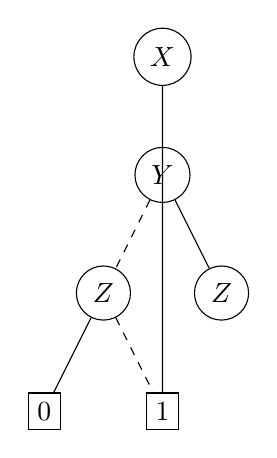
\begin{tikzpicture}

	[level 1/.style={sibling distance=33mm},
	 level 2/.style={sibling distance=23mm},
	 level 3/.style={sibling distance=16mm}]
	\node[circle, draw] (X) {$X$}	 
		child {node[circle, solid, draw] (Y) {$Y$} [dashed]
			child {node[circle, solid, draw] (Z1) {$Z$} [dashed]
				child {node[rectangle, solid, draw] (0) {0} [solid]}
				child {node[rectangle, solid, draw] (1) {1} [dashed]}}
			child {node[circle, solid, draw] (Z2) {$Z$} [solid]}};
	\draw[solid] (X) -- (1); 
\end{tikzpicture}

%\includegraphics[scale=•]{•}

\caption{The BDD for $f = $ with variable order $[]$ (left), and the SDD respecting the right-linear vtree inducing the same order (right)}
\label{fig:bdds_are_sdds}
\end{figure}

A very general consequence of this is that any application of BDDs in computer science could be implemented using SDDs instead, as it would retain the attractive properties of BDDs while benefiting from the potential reduction in size that SDDs present. In the more specific case of this project, we will see in a later chapter that this correspondence was extremely useful in helping us compare the efficiency of SDDs with that of BDDs in model checking: by restricting our SDD implementation to right-linear vtrees, we were able to compare both programs more accurately by taking into account the overhead due to the difference in \textit{implementation} (as opposed to a difference in size between the two structures -- we knew these were the same!).


\section{Implementation}

This chapter is devoted to the implementation of the model checker itself. We start by giving an overview of the existing code base and libraries upon which it relies, before presenting the important design decisions and algorithms, and finally discussing the challenges that occured during the implementation of this new model checker. 

\subsection{Preliminary I: The SDD Package}

\subsubsection{Description}

\textit{The SDD Package} is a C library which can be used to create and manipulate SDDs. It was developed at UCLA by the Automated Reasoning group, who first introduced SDDs. Its current version is 1.1.  


The SDD Package API contains most of the functions required for the use of SDDs in model checking. This includes basic manipulations such as conjunction, disjunction, and negation of Boolean functions represented by SDDs, conditioning a function on a literal, and quantifying out variables (the SDD equivalent of $\exists$ and $\forall$). Additionally, the API makes possible a number of operations on vtrees, including \textit{rotating }and \textit{swapping} (these are crucial for navigating the space of vtrees in the context of SDD minimisation, see below for details). 

The \textit{SDD manager} is the focal point for all the SDD operations in the program. It is there to ensure that all SDDs in the program have been built with respect to the same vtree, and it handles SDD conversions in the case of a vtree modification. It also gives the user access to a number of statistics, helpful for tracking a program's memory usage or the size of some SDD nodes. 

\subsubsection{Standard Vtrees}
\label{std_vtrees}

Four different ``classes" of vtrees are pre-implemented in the SDD package, i.e. can be created in one function call, provided a variable order is supplied. 
They are:
\begin{itemize}
\item right-linear: all left children are leaves
\item left-linear: all right children are leaves
\item balanced: the vtree is a balanced binary tree, i.e. both children of a node have the same number of leaves (if total number is even)
\item vertical: every node has a leaf child, which is alternatively the right child or the left child
\end{itemize}
Throughout this report we refer to these as the \textit{standard} vtrees. An example of each is given in Figure~\ref{fig:std_vtrees_example}.

\begin{figure}
\centering
\includegraphics[scale=0.4]{rightlinearABCD.png}
\quad
\includegraphics[scale=0.4]{balancedABCD.png}
\quad
\includegraphics[scale=0.4]{leftlinearABCD.png}
\quad
\includegraphics[scale=0.4]{verticalABCDE.png}
\caption{The four standard vtrees, in order: right-linear, balanced, left-linear, and vertical.}
\label{fig:std_vtrees_example}
\end{figure}

\subsubsection{Dynamic SDD Minimisation}
\label{sdd_dao_algo}
One particularly important feature of the SDD Package is \textit{dynamic SDD minimisation}. When enabled, this feature automatically attempts to minimise the size of a manager's SDD nodes by searching for a better vtree. Unfortunately this is not always a more efficient solution as searching the space of vtrees is a very lengthy process: there are $\frac{(2n -2)!}{(n-1)!}$ distinct vtrees over $n$ variables!

An vtree search algorithm was proposed in \cite{sdd_3} for more efficient dynamic minimisation of SDDs. This algorithm relies on three standard binary tree operations: left-rotation, right-rotation, and swap; these operations are sufficient for navigating the space of all vtrees \cite{knuth}.
The following example shows in what way these operations affect vtrees: 
\begin{example}
take a vtree with 4 nodes
\end{example}

We now give an informal description of the algorithm in \cite{ recursive calls on $v_l$ and $v_r$. We then consider two subtreesdd_3} (the one implemented in the SDD Package). We start with a vtree node $v$ (typically, the current vtree of the manager). The algorithm first makes two recursive calls on the children of $v$, ensuring that their structure is optimal. 
It then considers two vtree fragments of $v$, the \textit{l-vtree} and the \textit{r-vtree}. As shown on Figure~\ref{fig:lrvtrees}, each of these is a binary tree with 3 leaves (which might not be leaves in $v$). The algorithm attempts to compute the 24 distinct vtree fragments obtained by applying rotations and swaps to the l- and r-vtrees, and then selects the one leading to the best reduction in size for the SDD nodes depending on $v$. 

For each of the three vtree operations, users of the SDD package can set limits on the time needed to compute them, and the increase in size that they induce; this means that not all 24 vtree fragments above are necessarily computed. 

\subsubsection{Comparison with CUDD}

CUDD is the C$++$ BDD library used by MCMAS (see below) for BDD manipulation, and it is therefore our reference for all practical comparisons between SDDs and BDDs. 

Here we simply give an account of the differences between  CUDD and the SDD package, in order for our comparisons to be fair: we are interested in the relative efficiency of the data structures, not the packages, and therefore it is important that we take into account any differences in design and implementation. 

Fortunately, the libraries have a very similar flavour. For instance both are organised around a manager handling all internal operations. A few differences are worth mentioning:
\begin{itemize}
\item Both libraries have an automated garbage collection feature, and both are based on node reference counts. However the SDD Package requires users to manually increment and decrement the reference counts of each SDD node they create, whereas in CUDD this is optional (MCMAS doesn't use it). 
\item In the SDD Package the automated garbage collection and dynamic minimisation features are not independent, i.e. one cannot be enabled without the other being too. This means that when experimenting with SDDs without dynamic minimization, we find that a lot of unused nodes are kept in memory, sometimes preventing the program from generating any more SDDs in an efficient way (once the memory has run out, which happens relatively often in model checking when no garbage collection takes place). This is not the case in CUDD. 
\item An important difference in implementation is in the \texttt{exist()} function which relaxes the constraint on a variable $x$ in a function $f$, returning $f|_x \lor f|_{\lnot x}$. 
To do write more about exist
\end{itemize}
\label{gc}

\subsection{Preliminary II: MCMAS} 


MCMAS (Model Checker for Multi-Agent Systems) is a BDD-based model checker written in C$++$, which was developed, and is currently maintained at Imperial College in the Verification of Autonomous Systems group. It was specifically designed for the verification of multi-agent systems, and users can write system descriptions in a language called ISPL (Interpreted System Programming Language), whose syntax is very much inspired from the definition of interpreted systems (\ref{IS}). In order to better understand the implementation of the model checker, the reader is strongly advised to start by getting an overview of the main components in an ISPL file. For this purpose we supply a full example of an interpreted system encoded in ISPL: the \textit{Bit Transmission Protocol}, available in the appendix. ISPL is a fairly straightforward language, we therefore will not be spending any more time describing it here, but should anything remain unclear, the reader is refered the MCMAS User Manual \cite{mcmas}.



The model checker built for this project is (for a large part) based on the MCMAS code base. In this section we outline some of the MCMAS internal implementation details in order to help the reader understand the steps undertaken when replacing BDDs with SDDs. Moreover, MCMAS will be the basis of our BDDs vs. SDDs comparisons in the next chapters so it is important that the reader understand the different configuration options.

\subsubsection{Important Classes and Methods}
\label{MCMAS_steps}
The ISPL parser in MCMAS creates a model of the system using the following important classes: 
\begin{itemize}
\item \texttt{basic\_agent}: an agent in the system, consisting of a protocol, an evolution, a set of variables and a set of actions
\item \texttt{evolution\_line} and \texttt{protocol\_line}: a line in the evolution or in the protocol of an agent, consisting of a Boolean expression and an assignment or (respectively) an action
\item \texttt{bool\_expression} and \texttt{assignment}
\item \texttt{variable}, \texttt{basic\_type}, \texttt{int\_value}, \texttt{enum\_value}, \texttt{bool\_value},  \texttt{rangedint}, \texttt{atomic\_proposition}, \texttt{laction}: agent variables, their types and their values
\item \texttt{modal\_formula}: a CTLK formula to be checked in the model.
\end{itemize}
Throughout the model checking procedure the \textit{BDD parameters} are carried by the program and passed as argument to the various methods. They are encapsulated in a structure (\texttt{struct bdd\_parameters}) and contain all the important data required by the algorithm, in particular: 
\begin{itemize}
\item three vectors \texttt{v}, \texttt{pv}, and \texttt{a}, containing the Boolean variables used in the model for encoding states, next states, and actions respectively
\item a vector \texttt{vRT}, containing for each agent the BDD for its transition relation 
\item the BDD \texttt{in\_st} representing the set of initial states, and (once computed) the BDD \texttt{reach} for the reachable state space
\item a pointer to the BDD cache
\item a vector \texttt{is\_formulae} containing the \texttt{modal\_formula} objects for each CTLK formula to check
\end{itemize}
MCMAS is (quite literally) an implementation of the model checking algorithm described in \ref{explicit}. However, as a symbolic model checker it also contains procedures for encoding protocols, transition relations, sets of states and actions, etc., and in fact these constitute a very large part of the code. 
We list the main steps in the execution of the program:
\begin{enumerate}
\item Parse ISPL file, allocate variables and set up CUDD (see \ref{variable_allocation} below)
\item Compute the BDD for the global transition relation
\item Compute the BDD for the reachable state space 
\item For each modal formula $\varphi$, compute
\texttt{SAT($\varphi$)} and check that it is a subset of $I$
\item Output result and free memory
\end{enumerate}


\subsubsection{Variable Allocation}
\label{variable_allocation}
Variable allocation is the process of allocating manager variables (created with the manager) to agents and determining the various sets of variables needed for symbolic representation within each agent: state variables, primed state variables (a copy of the state variables representing the \textit{next }states), and action variables.

For each agent, MCMAS first computes the number of variables needed in each of the aforementioned sets by calls to the functions \texttt{state\_BDD\_length()} and \texttt{action\_BDD\_length()}.

The \texttt{basic\_agent} functions \texttt{allocate\_BDD\_2\_variables()} and \texttt{allocate\_BDD\_2\_actions()} are then used for variable allocation: they assign a portion of both \texttt{v} and \texttt{a} to each agent, giving them start and end \textit{indices}. Note that this forces all of an agent's state variables (and similarly, action variables) to be next to each other in \texttt{v} (and similarly, \texttt{a}). 

It may seem confusing that variable allocation happens before the user has been able to select a particular variable order, but in fact no actual variables have yet been allocated, only their position in the arrays. The user's choice will then affect the way the \textit{manager}'s variables are dispatched across \texttt{a}, \texttt{v}, and \texttt{pv}. 

In MCMAS, the user can choose between four \textit{standard} different variable orders. We take the time to present them here, not only because of the impact that this choice has on the overall performance, but also for reference in the future chapters (where we compare these orders with various SDD vtrees).

\subsubsection{Standard Variable Orders}
 \label{std_orderings}
Suppose MCMAS is running on an example requiring $n$ state variables denoted $x_1, ..., x_n$, and $m$ action variables denoted $a_1, ..., a_m$. By definition there are $n$ primed state variables (the next state is a state, so it can be represented with the $n$ state variables), these are denoted $x_1', ..., x_n'$. 
Suppose also that there are $k$ agents, and that for each $i$, agent $i$ has been allocated variables $x_{i_1}, ..., x_{i_{n_i}}$, $x_{i_1}', ..., x_{i_{n_i}}'$ and $a_{j_1}, ..., a_{j_{m_i}}$, for some $n_i, m_i \in \mathbb{N}$ and where $i_1, ..., i_{n_i}$ and $j_i, ..., j_{m_i}$ are sequences of consecutive integers.



The manager will then have $2n + m$ variables in total, and the following are the possible four ordering options with respect to which BDDs will be constructed throughout the process:
\begin{itemize}
\item Ordering option 1:
$$x_1, ..., x_n, x_1', ..., x_n', a_1, ..., a_m$$
\end{itemize}
In options 2 to 4, variables are ordered using the agent order, so that we get an ordering of the form $$ \mbox{variables for agent } 1, \mbox{variables for agent } 2, ...,  \mbox{variables for agent } k.$$ 
The difference lies in the way variables are ordered within each agent set:
\begin{itemize}
\item Ordering option 2:
$$
 \mbox{variables for agent } i = x_{i_1}, x_{i_1}', x_{i_2}, x_{i_2}',..., x_{i_{n_i}}, x_{i_{n_1}}', a_{i_1}, ..., a_{i_{m_1}}
$$
\item Ordering option 3:
$$
 \mbox{variables for agent } i = x_{i_1}, ..., x_{i_{n_i}},a_{i_1}, ..., a_{i_{m_1}}, x_{i_1}', ..., x_{i_{n_1}}'
$$
\item Ordering option 4:
$$
 \mbox{variables for agent } i = x_{i_1}, ..., x_{i_{n_i}}, x_{i_1}', ..., x_{i_{n_1}}', a_{i_1}, ..., a_{i_{m_1}}
$$

\end{itemize}

\subsubsection{Algebraic Decision Diagrams}

MCMAS supports bounded integer variables (e.g. \texttt{x : 0..3}), and allows Boolean conditions to be numeric identities (e.g. \texttt{(x > 2)} or \texttt{(x + y = 3)} for integer vars \texttt{x} and \texttt{y}). 

If an agent has an integer variable with a large range of values, then the number of Boolean variables needed to represent its state is also large (if variable \texttt{x} has $n$ possible values, the corresponding agent needs at least $\log_2(n)$ state variables). 

To avoid this, MCMAS uses alternative data structures called \textit{algebraic decision diagrams} (ADD, \cite{add}) to represent these variables and expressions. The CUDD manager also handles ADDs, and the ADD variables needed are stored in global vectors \texttt{addv} and \texttt{addpv}.

As there is no SDD equivalent for ADDs (yet!), our model checker does not support examples containing numerical values and expressions.
Note that all these examples \textit{could} technically be implemented in ISPL so that our model checker supports them, by simply replacing an integer range by an \textit{enum} containing all the possible values that the variable can take: for example 
$$\texttt{x : 0..3} $$
could be declared as $$\texttt{x : \{zero, one, two, three\}}$$
and expressions such as $$\texttt{if (x > 1)}$$ could be translated to $$\texttt{if (x = two) or (x = three)}.$$
With ADDs being beyond the scope of this project, we did not study them further (in particular we did not look into the ADD reduction done by CUDD in the background), and therefore thought better not to implement this to keep the comparison fair between MCMAS and our model checker. 

\subsection{A Model Checker Based on SDDs}

\subsubsection{Adapting MCMAS}

We implemented a model checker for multi-agent systems entirely based on SDDs for symbolic representations. 

Our starting point was the MCMAS source code, in which we proceeded to replace every call to CUDD with equivalent calls to the SDD Package. Throughout, we managed the reference counts of our SDD nodes by calls to \texttt{sdd\_ref()} and 
\texttt{sdd\_deref()}. Note that this often requires the introduction of temporary nodes; specifically, this occurs when updating the value of a node based on its previous value. For instance, the CUDD statement 
\begin{verbatim}
// f, g are BDDs
f = f * g; 
\end{verbatim}
setting the value of $f$ to be the conjunction of the BDDs for $f$ and $g$, becomes
\begin{verbatim}
// f, g are SddNode*
SddNode* tmp;
f = sdd_conjoin(tmp = f, g, manager);
sdd_ref(f, manager);
sdd_deref(tmp, manager);
sdd_deref(g, manager); // (if this is the last time we use g)
\end{verbatim}
This is to ensure that the previous SDD node pointed to by $f$, which the code can no longer access, is garbage collected. As a more complete example we provide the code for the \texttt{compute\_reach()} function in appendix (To Do).

The main steps of our model checker are the same as those of MCMAS described in \ref{MCMAS_steps}, and therefore the important functions which had to be adapted for SDDs are: 
\begin{itemize}
\item the functions \texttt{encode\_protocol()}  and \texttt{encode\_evolution()} for each agent, used to compute the global transition relation
\item the \texttt{compute\_reach()} function for computing the SDD representing the global reachable state space
\item the \texttt{check\_formula()} method (the implementation of \texttt{SAT})
\end{itemize}

Additionally, new data types and functions had to be defined in order to deal with the SDD-specific aspects of the program. We replaced the MCMAS BDD parameters by our own \textit{SDD parameters} (see appendix) containing the results of the variable allocation process in three different vectors: \texttt{variable\_sdds}, \texttt{primed\_variable\_sdds}, \texttt{action\_variable\_sdds}.

\subsubsection{Existential Quantification}

Recall  (\ref{exist}) that the model checking algorithm relies on the functions $\mbox{pre}_\exists$ and $\mbox{pre}_\forall$, which themselves depend on existential quantification, or the process of relaxing the constraint on one or more variables in a function. 

In CUDD, the function responsible for existential variable quantification is \texttt{Cudd\_bddExistAbstract()}. This takes as input two BDDs $f$ and $c$, and returns the BDD for $f$ after existential quantification of all variables in $c$. The implementation of this function is based on the following recursive algorithm called \texttt{restrict}, originally described in \cite{unified_framework}: 

\begin{lstlisting}[mathescape]

function restrict(f, c):
// pre:$ \mbox{ c != } \bot$ and variables of c are all variables of f
  if c = $\top$ or f = $\bot$ or f = $\top$
    return f
  x := top variable in f // the root of the BDD
  if (x = top variable in c)  
    return (restrict(f$|_{\mbox{x}}$, c$|_{\mbox{x}}$) $\lor$ restrict(f$|_{\lnot\mbox{x}}$, c$|_{\mbox{x}}$))
  else // x does not appear in c
    return (x $\land$ restrict(f$|_{\mbox{x}}$ , c)) $\lor$ ($\lnot$x $\land$ restrict(f$|_{\lnot\mbox{x}}$ , c))
end
$\\$
\end{lstlisting}

In the context of symbolic model checking, existential quantification of a set of variable $X$ from a function $f$ can be done in CUDD by a call to \texttt{Cudd\_bddExistAbstract(f, c)}, where \texttt{f} is the BDD for $f$ and \texttt{c} is a function essentially depending on all the variables in $X$ (in MCMAS \texttt{c} is set to be the conjunction of all the variables in $X$).

In the SDD Package, existential quantification can only be done one variable at a time, by calling \texttt{sdd\_exists(x, f, manager)} which returns $\exists x f$. Our first solution was to iteratively call this function on every variable in $X$, but our first experiments revealed that this method was very slow. We therefore implemented the above algorithm in our model checker as an attempt to reduce computation time:

\begin{lstlisting}[mathescape]

SddNode* restrict_sdd(SddNode* f, SddNode* c, SddManager manager) 
{
  if(sdd_node_is_false(c)) // not allowed
    return NULL; 
  if(sdd_node_is_true(c) || sdd_node_is_false(f) || sdd_node_is_true(f))
    return f;
  SddLiteral x = get_top_variable(f);
  SddLiteral y = get_top_variable(c);
  if (x == y) {
    SddNode* res1 = restrict_sdd(sdd_condition(x, f, manager), sdd_condition(x, c, manager), manager);
    SddNode* res2 = restrict_sdd(sdd_condition(-x, f, manager), sdd_condition(x, c, manager), manager);
    return sdd_disjoin(res1, res2, manager);
  } else {
    SddNode* res1 = restrict_sdd(sdd_condition(x, f, manager), c, manager);
    SddNode* res2 = restrict_sdd(sdd_condition(-x, f, manager), c, manager);
    return ite(sdd_manager_literal(x, manager), res1, res2, manager);
  }
}

\end{lstlisting}
In the code above, \texttt{ite} refers to an implementation of the ITE (If-Then-Else) operator on Boolean functions, namely $$\mbox{ITE}(f, g, h) = (f \land g) \lor (\lnot f \land h).$$

Another point worth discussing is the notion of ``top variable" for an SDD. In a BDD, this is unambiguously refering to the variable with which the root is labelled, and this choice of variable for the start of the algorithm is clearly induced by the conditioning algorithm on BDDs, which consists in removing the \textit{false} outcoming edge for each node labelled with the variable in question -- if this is the top variable, then this amounts to simply removing the right (or left) subtree of the BDD. 

In an SDD however, this is not so obvious: 

to do: talk about \texttt{sdd\_condition()} and the performance of our implementation.



\subsection{SDD-Specific Features}

\subsubsection{Vtrees and Variable Orders}

Recall that in the SDD Package, the use of the standard vtrees is only possible when a variable order is supplied. For convenience, we implemented the four standard MCMAS variable orders in our model checker, for use with one of the standard vtree, thereby making 16 different vtrees available. These orderings are implemented within the \texttt{get\_var\_order()} function, whose code is documented in appendix. 

As explained in the evaluation section of this report, these 16 vtrees quickly proved insufficient for our purposes, and being able to create our own ``non-standard" vtrees became crucial for the progress of the project.  
The SDD Package API is lacking some basic functions in that area, most probably because it is generally sufficient for users to rely on the standard vtrees, together with the dynamic minimisation feature. There are, for example, no ways of constructing a vtree bottom-up, as one would construct an SDD node. To create our own customised vtrees, we had the two following options:
\begin{itemize}
\item Generate a variable order to create one of the standard vtrees, and apply swaps, left- and right-rotations until the vtree obtained is the desired vtree
\item Generate a \textit{vtree format} text file and use \texttt{sdd\_vtree\_read()} to create a \texttt{Vtree} object. According to the SDD manual, this file format is normally used to save vtrees to file in order to re-use them in the future. The function \texttt{sdd\_vtree\_save\_to\_file()} is the way to generate the file from an existing vtree.

\end{itemize}
We chose the second option, simply because it seemed more convenient than computing the set of operations to apply to get from one vtree to another. The vtree format, without being particularly readable, has the advantage of being relatively simple in syntax and therefore easy to generate. 

The API of the SDD Package was clearly not designed to edit and manipulate vtrees practically, so as a replacement we created a new tree structure, the \texttt{vtree\_node}, defined thus: 
\begin{verbatim}
struct vtree_node 
{
  // the children
  vtree_node * left; 
  vtree_node * right;
  // more data for file generation
  int size;
  bool isleaf;
  int id;
};
\end{verbatim}

This very simple structure significantly facilitated the process of constructing vtrees. We could simply create a leaf \texttt{vtree\_node} for each variable needed, and construct the vtree bottom-up. Observe that the variables themselves are not stored; this is because we organise the nodes so that each variable is \textit{one more} than the ID of the leaf which contains it (IDs start from 0 in the file, whereas variables are numbered from 1 in the SDD manager).

 The function \texttt{vtree\_node\_get\_file\_content()} was written to recursively return the string representing the \texttt{vtree\_node} in the file format required by \texttt{sdd\_vtree\_read()}. The code for the function, as well as an example, can be found in the appendix (To do). 

In practical applications, the number of variables is not known in advance but we still need a way of generating the vtree dynamically. To this aim, we wrote the \texttt{create\_vtree()} function which is called in the program as soon as the number of variables needed is known, but \textit{before} the SDD manager is created, so that the vtree produced can be used during its initialisation -- note that this is only possible since our vtree is not based on actual variables but on a temporary structure which does not involve the manager. 

To use \texttt{create\_vtree()}, we need to pass it the number of variables that the vtree should consist of, as well as the desired \textit{vtree type}. This is an integer corresponding to one of the various vtrees which we implemented: vtree types 1-4 correspond to the standard vtrees defined in \ref{std_vtrees}, whereas types 4-8 are ``new" vtrees which we found to have more potential in the context of model checking. We leave out the details for now and use the evaluation section to describe the process leading to their discovery. 

\subsubsection{Dynamic Vtree Search in Multi-Agent Systems}

In \ref{sdd_dao_algo}, we described the dynamic minimisation algorithm implemented in the SDD Package. This algorithm is focused on a complete restructuring of the manager's vtree in order to minimise the size of its SDD nodes. 

Early experiments with this algorithm revealed large 


However, in multi-agent systems, it is 


\subsection{Software Engineering Issues and Challenges}

Here we explain some of the challenges faced during the implementation of the model checker. 

\subsubsection{Garbage Collection}

As described in \ref{gc}, the SDD Package has a automatic garbage collection feature based on reference counts, but it leaves the referencing and dereferencing of nodes to the user. 

If not done properly, node referencing can lead to issues such as unwanted garbage collection, dead nodes kept in memory, or dead node dereferencing, all of which being very undesirable (but for different reasons).

This forced the constant track-keeping of node reference counts and required more debugging time. Nonetheless, it is important to mention that the manual referencing and dereferencing of nodes is probably more efficient in the long run than if the SDD manager had to do it in the background, which would require more thinking on its part.

\subsubsection{Comparing SDDs and BDDs}

The goal of this implementation was to build an SDD-based model checker which produced the same results as MCMAS in all circumstances. We needed to make sure that the Boolean functions representating our sets of states and transition relations were the same at each step of our model checking algorithm. Unfortunately, there is no convenient and precise way of programmatically comparing an SDD with a BDD. 

The only \textit{exact} method available is to look at the Boolean function corresponding to each data structure, and compare these. However, due to their syntactic differences, it had to be done using a SAT checker (we used \cite{minisat}), which is a good solution for small functions but becomes impractical very quickly when the number of variable exceeds about 20 (which happens in all non-trivial cases).  

An useful alternative is to construct the SDD with respect to a right-linear vtree and the BDD with the equivalent variable ordering (see \ref{bdds_are_sdds} for details), to ensure that the resulting structures are comparable. We then have two options:
\begin{itemize}

\item Compare the graphical representation of each data structure, provided by both APIs via a DOT file \cite{dot}. An image is often enough to tell if two representations are not equivalent, but in the case where they are, it can be a very long process to manually verify it.
\item Compare the size (i.e. the number of nodes) of each structure. Again, most of the time two non-equivalent representations have very different sizes, but representations with comparable sizes are not necessarily equivalent (note that due to the way SDD and BDD nodes are counted, the size of a BDD is not exactly the same as the size of the equivalent SDD so this method is not 100\% conclusive either).

\end{itemize}
 This second option is nonetheless the only available solution in the case of very large SDDs and BDDs, which explains the difficulty in debugging larger examples.

Reflecting back on this issue, it would have been much less time-consuming to write a small logic equivalence tool ensuring that the Boolean functions obtained from two equivalent data structure was not only equivalent, but also \textit{syntactically equal}, to reduce the problem to a simple comparison of strings. We did not anticipate enough the amount of work that would be required when debugging the model checker.

\subsubsection{Correctness}

It is a little ironic that verifying correctness of a verification software was such a complicated task. Due to the reasons mentioned above, we had to use a few simple tricks to make sure that our code was indeed an implementation of the model checking algorithm. 

The first technique we used was that of comparing the \textit{output} of our model checker with that of MCMAS, on the set of examples that we had available (see \ref{ispl_examples} for a detailed description of these examples). Once we were certain that these were identical (so no obvious bugs existed), we did a more thorough search to ensure that there was nothing wrong with the code. 

write more about this

Although our set of examples was relatively diverse, it certainly did not cover the whole range of expressions, data types, etc. available in ISPL, nor did it use the full set of CTLK connectives that ISPL supports.



\section{Evaluation (?)} 


\subsection{Setup and Evaluation Plan}

\subsubsection{Evaluation Strategy}

The ultimate objective of this project was either to establish, or to refute SDDs (in their current state) as serious competitors to BDDs in model checking. The obvious plan for quantitative analysis was to do a side-by-side comparison of our model checker and MCMAS on a series of examples, and conclude. However, in order to provide a fair comparison we had to ensure that both structures were performing ``at the best of their abilities". 

There are suggested methods for the use of BDDs in model checking, in particular concerning initial variable orders~\cite{bdd_heuristics}. For the specific case of MCMAS we observe that the standard order number 2 (see \ref{std_orderings}) \textit{often} yields the best results.
On the other hand, SDDs had not yet been explored in the context of model checking, and consequently no heuristics existed. 

Through this evaluation we planned to remediate this by investigating various vtree constructions and comparing them with MCMAS. 

To start with, we decided to focus on the issue of \textit{static} vtree generation, for the situation where the vtree has to be determined \textit{before} SDDs are constructed, as opposed to continuously modified as the construction process happens (this is called \textit{dynamic} minimisation). 

Although it may seem like wasted effort, the importance of static vtree generation is non-negligible, for two reasons: firstly, it helps us understand what aspects of the vtree have the greatest impact on the final SDD; secondly, even though dynamic minimisation is generally the most efficient technique, it can also be a very time-consuming process which some applications might find less practical. 

After this first investigation, we planned to look at the performance of SDDs when enabling the dynamic minimisation feature of the SDD Package, and compare it to BDD dynamic variable reordering as implemented in MCMAS.

We hoped that both of these analyses (static and dynamic) would provide enough information to know whether or not SDDs (as implemented in the SDD Package) are suitable for model checking multi-agent systems.

	\subsubsection{Example Models}
	\label{ispl_examples}
\begin{itemize}
\item Bit transmission problem 
\item Dining Cryptographers
\item Prisoners' dilemma 
\item NSPK - 
http://en.wikipedia.org/wiki/Needham-Schroeder\_protocol
\end{itemize}

also: choice of examples, why parametrised 
\subsubsection{Machine, Configurations, Benchmarking Process} 



\subsection{Comparisons with Standard Vtrees under Static Vtree Generation}

We started our investigation by experimenting with the standard vtrees, i.e. those pre-implemented in the SDD package, namely right-linear, left-linear, balanced, and vertical. Recall that this first investigation was focused exclusively on static vtree generation

\subsubsection{Right-Linear Vtrees} 

\begin{itemize}
\item why it's important
\item data: it's much slower
\item various orderings make no difference but performance changes linearly compared to BDD orderings (which makes sense) -- does it??
\item analysis
\item for rest of static evaluation: if we find an improvement on right-linear vtrees, it can be an improvement on bdds if package performances are ever the same
\end{itemize}


Recall that BDDs are structurally identical to SDDs build using a right-linear vtree, and the same variable ordering (\ref{bdds_are_sdds}). Experimenting with this particular type of vtrees was therefore of significant importance, as it would allow us to compare both data structures at the same level.  

The data in the table \ref{} below corresponds to runs of MCMAS vs...

$$DATA$$

During this first phase of the investigation, it became very quickly apparent that SDDs were \textit{significantly }). 
When investigating further, the origin of the overhead slower than BDDs; their computation time even appeared to grow exponentially compared to BDDs (to do: this is just conjecture). 




\subsubsection{Other Standard Vtrees}

\begin{itemize}
\item data: it's much much slower: these vtrees are not appropriate.. except maybe balanced *sometimes*. 
\item reason: too much weight on left child nodes of vtree 
\end{itemize}

\subsubsection{Towards a Better Vtree: Observations}

\begin{itemize}
\item seems standard vtrees are not good enough with any orderings 
\item where is the overhead and what would make it decrease? 
\item we run the dynamic minimisation feature, what we find: 
\begin{itemize}
\item vtrees are pseudo-right-linear
\item how are variables arranged
\item look at how vtree changes during the process
\end{itemize}
\item if we come up with new static heuristics, they need to make sense and we should be able to generate them automatically from the model 
\end{itemize}


\subsection{Static Experiments with Alternative Vtrees}

\subsubsection{A First Attempt}

inspired from MCMAS orderings we split the variables by agent

\subsubsection{An Upper Bound on Subtree Size}

important to explain why this improves computation times

\subsubsection{Various Vtree Characteristics and Their Impact}

\begin{itemize}
\item changing the way variables are allocated to subtrees
\item changing variable order \textit{within} subtrees and subtree type
\item changing subtree order, and possibly adapting compute\_reach algorithm
\item 

\end{itemize}

We aim to find an initial vtree leading to faster computations. We notice that whatever the initial vtree, dynamic reduction algorithms always result in a particular type of vtree, which we call \textit{pseudo-right-linear}. 
All our experiments are with pseudo-right-linear vtrees.
\begin{itemize}
\item vtree experiment 1 (option 5): one balanced subtree per agent. 

This does \textit{not} work well.
\item vtree experiment 2 (option 6): We set a maximum size for agent subtrees. An upper bound of $\log_2(n^2)$ (where $n$ is the number of vars) has proved relatively efficient. If an agent has more variables then we create more subtrees for it. Variables of a subtree come from the same agent. Subtrees are balanced, and we experiment with different orderings for them. We observe that the best results are obtained when two principles are followed: action variables are close to each other in the subtree (i.e they alone form a balanced vtree of size \texttt{action\_count}) and states variables are 
paired with their primed counterpart. (TODO: confirm this!)

\item vtree experiment 3 (option 7): Each subtree contains one variable for each agent, as well as its corresponding primed variable. Action variables for each agent form their own subtree. We order state subtrees 'largest to smallest' and put action subtrees at the bottom. This seems to be the best ordering but TODO need to try: intercaler actions/states.

\item vtree experiment 4 (option 8): Think of something! 

\end{itemize}

\subsection{Using Dynamic Reordering and Minimisation}

\subsubsection{Initial Observations}

Raw data with all examples and stuff 

\subsubsection{Experiments}

\begin{itemize}
\item 
\item 
\end{itemize}

\subsubsection{Grouping Variables}
new vtree search method 
\subsection{Summary}

review of best techniques and heuristics

\section{Conclusion and future work}

\subsection{Review}

\subsection{Future work}

Missing features will be counterexample/witness generation, and checking for deadlock or model overflow. Also being able to check ATL formulas.
At some point I would like to have a go at implementing an ADD equivalent for SDDs.
-> Call \texttt{sdd\_apply()} on a reduced vtree


\begin{thebibliography}{9}


\bibitem{sdd_1}
A. Darwiche:\emph{ SDD: A New Canonical Representation of Propositional Knowledge Bases}, 2011.

\bibitem{sdd_2}
A. Darwiche, A. Choi, Y. Xue: \emph{Basing Decisions on Sentences}, 2012.

\bibitem{sdd_3}
A. Darwiche, A. Choi: \textit{Dynamic Minimization of Sentential Decision Diagrams}, 2013.

\bibitem{compilation_map}
  A. Darwiche, P. Marquis:
  \emph{A Knowledge Compilation Map}, 2002.

\bibitem{trees_of_bdds}
S. Subbarayan, L. Bordeaux, Y. Hamadi:\textit{
Knowledge Compilation Properties of Tree-of-BDDs}, 2007.

\bibitem{bdd_trees}
K. L. McMillan:\textit{ Hierarchical representations of discrete functions, with application to model checking, 1994.
}

\bibitem{logic_in_computer_science}
 M. Huth, M. Ryan, 
\emph{Logic in Computer Science},
Cambridge University Press, 2004.

\bibitem{knuth} D. E. Knuth, \textit{The Art of Computer Programming, Volume
4, Fascicle 2: Generating All Tuples and Permutations}, Addison-Wesley Professional, 2005.

\bibitem{add}  R. I. Bahar, E. A. Frohm, C. M. Gaona, G. D. Hachtel, E. Macii, A. Pardo, F. Somenzi:\textit{
Algebraic decision diagrams and their applications}, 1993.

\bibitem{bdd_heuristics} M. Rice, S. Kulhari:\textit{ A Survey of Static Variable Ordering Heuristics for Efficient BDD/MDD Construction}, 2008.

\bibitem{bryant} R. E. Bryant: \textit{Graph-Based Algorithms
for Boolean Function Manipulation}, 1986.

\bibitem{ctl*}  	E. A. Emerson, J. Y. Halpern:\textit{
``Sometimes" and ``not never" revisited: on branching versus linear time temporal logic}, 1986.
	
\bibitem{ctlk}R. Fagin, J. Y. Halpern, Y. Moses, M. Y. Vardi: \textit{Reasoning about Knowledge}, 1995.

\bibitem{unified_framework} O. Coudert, J-C. Madre: \textit{A Unified Framework For the Formal Verification of Sequential Circuits}, 1990.

\bibitem{MCMAS_website} MCMAS webpage, http://vas.doc.ic.ac.uk/software/mcmas/

\bibitem{CUDD_website} CUDD Package webpage, http://vlsi.colorado.edu/~fabio/CUDD/

\bibitem{SDD_website} SDD Package webpage, http://reasoning.cs.ucla.edu/sdd/

\bibitem{minisat} David A. Wheeler's MiniSAT solver,  http://www.dwheeler.com/essays/minisat-user-guide.html

\bibitem{dot}Graphviz DOT, http://www.graphviz.org/Documentation.php

\bibitem{notes_303} A. Lomuscio, Software Engineering: Software Verifications, lecture notes (as taught in 2012-13)

\bibitem{notes_499} I. Hodkinson, Modal and Temporal logic, lecture notes (as taught in 2013-14)

\end{thebibliography}

\end{document}
